\documentclass[10pt,showpacs,preprintnumbers,amsmath,amssymb,nofootinbib,aps,prl,twocolumn,groupedaddress,superscriptaddress,showkeys]{revtex4-1}
\usepackage{graphicx}
\usepackage{dcolumn}
\usepackage{bm}
\usepackage[colorlinks=true,urlcolor=blue,citecolor=blue]{hyperref}
\usepackage{color}
\usepackage{listings}
\usepackage{subfig}
\usepackage{float}

\lstset{ %
  basicstyle=\footnotesize,        % the size of the fonts that are used for the code
  breakatwhitespace=false,         % sets if automatic breaks should only happen at whitespace
  breaklines=true,                 % sets automatic line breaking
  captionpos=t,                    % sets the caption-position to bottom
  deletekeywords={...},            % if you want to delete keywords from the given language
  escapeinside={\%*}{*)},          % if you want to add LaTeX within your code
  extendedchars=true,              % lets you use non-ASCII characters; for 8-bits encodings only, does not work with UTF-8
  frame=single,                    % adds a frame around the code
  keepspaces=true,                 % keeps spaces in text, useful for keeping indentation of code (possibly needs columns=flexible)
 % language=Python,                 % the language of the code
  morekeywords={*,...},           % if you want to add more keywords to the set
  numbers=left,                    % where to put the line-numbers; possible values are (none, left, right)
  numbersep=5pt,                   % how far the line-numbers are from the code
  showspaces=false,                % show spaces everywhere adding particular underscores; it overrides 'showstringspaces'
  showstringspaces=false,          % underline spaces within strings only
  showtabs=false,                  % show tabs within strings adding particular underscores
  stepnumber=1,                    % the step between two line-numbers. If it's 1, each line will be numbered
  tabsize=2,                       % sets default tabsize to 2 spaces
}


\begin{document}
\title{FYS3150 Computational Physics - Project 3}
\author{Nicholas Karlsen}


\begin{abstract}
  Looking at how n-coupled differential equations can be solved numerically using the Velocity-Verlet and Forward Euler algorithms for systems governed by Newtonian gravity. Found that the Forward Euler method falls short compared to the Velocity-Verlet method as it is non-conservative and requires a greater number of integration points to converge in the given system. There was also an unsuccessful attempt at reproducing the perihelion precession of mercury using a modified model in a 2-body system.
\end{abstract}

\maketitle


\section{Introduction}

  In this report we will take a look at two methods for solving Ordinary differential equations numerically, which is of great interest in physics as a lot of physical systems are governed by such equations, most of which lack closed form analytical solutions. In particular, we will look closely at how these numerical methods can be used to solve multi-body systems governed by Newton's law of gravity, which has no exact analytical solutions for $n\geq3$ bodies, as well as looking at a slightly altered model, which accounts for relativistic effects, this time restricting ourselves to a 2-body system.

  Therefore, i have developed a flexible object oriented class in python which solves systems of coupled differential equations using the Velocity-Verlet algorithm and the Forward Euler method, the source code of which can be found on my Github page at: \url{https://github.com/nicholaskarlsen/FYS3150}. 

\section{Theory, Algorithms and Methods}
  
  \subsection{Newton's law of universal gravitation}
    Between every body, there is a force of attraction inversely proportional to the square of their separation, or more precisely, the force acting on some body with mass $m$ due to a mass $m'$ is
    \begin{equation}
      \mathbf F = -G\frac{m m'}{|\mathbf r - \mathbf r'|^2}\mathbf{\hat{u}_{r-r'}}, \quad \mathbf{\hat{u}_{r-r'}} = \frac{\mathbf r - \mathbf r'}{\mathbf |\mathbf r - \mathbf r'|}
      \label{eqn:newton gravity}
    \end{equation}
    Where $G$ is the gravitational constant and $\mathbf r, \mathbf r'$ denote the position vectors of bodies with mass $m, m'$ respectively.

    Choosing the the 2D Cartesian coordinate system, let $\mathbf r - \mathbf r'= (x_{r}, y_{r})$, where the $r$ suffix denote that these coordinates are to be understood as the relative coordinates between bodies $m, m'$.
    Further, $|\mathbf r - \mathbf r'| = \sqrt{x_r^2 + y_r^2} = r$ is the distance between the two bodies.

    By Newtons second law, the acceleration on body 1 due to the gravitational pull of body 2 can then be written as
    \begin{equation}
      \mathbf a = \frac{1}{m}\mathbf F = -G \frac{m'}{r^2}\frac{(\mathbf r-\mathbf r')}{r} = -G\frac{m'}{r^2}\frac{\left(x_r, y_r\right)}{r}
    \end{equation}
    Written out component-wise in terms of the positions, we get the set of coupled differential equations

    \begin{equation}
      \frac{\partial^2 x}{\partial t^2} = -G\frac{m'}{r^2}\frac{x_r}{r}, \quad
      \frac{\partial^2 y}{\partial t^2} = -G\frac{m'}{r^2}\frac{y_r}{r}
    \end{equation}
    Similar, for 3 dimensions where $\mathbf r - \mathbf r' = (x_r, y_r, z_r), r=\sqrt{x_r^2 + y_r^2 + z_r^2}$.

    This force also forms a vector field, and the associated potential energy due it is
    \begin{equation}
      E_p(\mathbf r) = -G\frac{mm'}{r}
    \end{equation}
    The derivation of which is given in \cite{elem}, and elsewhere.
    From this, we can form an equation for the escape velocity of a body "trapped" in a gravitational field. Which is the velocity in which the Kinetic energy is greater or equal to the potential energy, that is
    \begin{equation}
      \frac{1}{2}m v^2 = G\frac{mm'}{r}
    \end{equation}
    Which leads to the expression
    \begin{equation}
      v_{escape} = \sqrt{\frac{2Gm'}{r}}
      \label{eqn:escapevel}
    \end{equation}

    A special solution to the differential equation \ref{eqn:newton gravity} is for the perfectly circular orbit, for which we can use the equations of circular motion and get exact analytical predictions very easily. 
    \begin{align}
    \begin{split}
      \frac{v^2}{r} &= G\frac{m'}{r^2}
      \\ v &= \sqrt{\frac{Gm'}{r}}
    \end{split}
    \end{align}
    where in this case, the speed $v$, as well as $r$ are expected to be constant quantities.

      \begin{figure}[h!]
        \center
        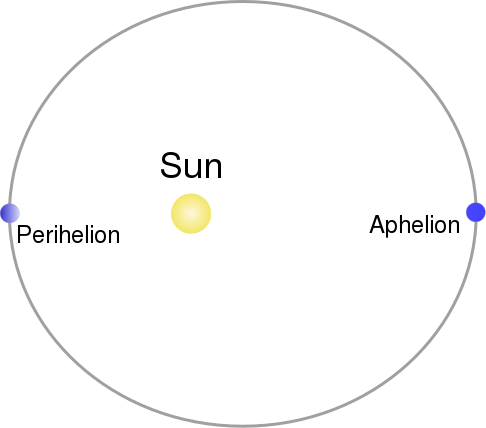
\includegraphics[width=4cm]{figs/486px-Perihelion-Aphelion.png}
        \caption{In an elliptic orbit, the closest and farthest points in the orbit is defined as the Perihelion and Aphelion respectively [\href{https://en.wikipedia.org/wiki/Perihelion_and_aphelion}{Image source}]}
        \label{fig:perhelion}
      \end{figure}

    
    \subsubsection{Relativistic Correction}

      The aforementioned model of gravity fails to predict the perihelion (see fig. \ref{fig:perhelion}) precession of mercury, which is observed to be $43"$ (arc seconds) per century \cite{problem_set}. 

      That is, the closed, uniform elliptical orbits predicted by the Newtonian model for gravity does not match with observations in Astronomy, where the perihelion of Mercury seems to shift its location over time. In fact, the perihelion precession of mercury was the first experimental confirmation of General relativity, the model of gravity developed by Albert Einstein which accurately predicts this phenomena.

      And so, a correcting factor accounting for the relativistic effects is added to Newtons model, and the magnitude of the gravitational force becomes \cite{problem_set}

      \begin{equation}
        |\mathbf F| = G \frac{m m'}{r^2}\left[1 + \frac{3l^2}{r^2c^2}\right]
        \label{eqn:relativistic correction}
      \end{equation}
      Where $l$ denotes the magnitude of the angular momentum of the orbiting body and $c$ the speed of light.
\subsection{Solving ODEs numerically}
  \subsubsection{Forward Euler}
    Consider a function $f(t)$, which derivative, $f'(t)$ is known and we want to find $f(t + \delta t)$. 
    Take the taylor expansion of $f(t + \delta t)$
    \begin{equation}
      f(t + \delta t) = f(t) + f'(t)\delta t + \frac{1}{2}f''(t)\delta t^2 + \dots + \frac{1}{n!}f^{(n)}(t)\delta t^n
    \end{equation}
    If we then truncate this series after the second term we get
    \begin{equation}
      f(t + \delta t) = f(t) + f'(t)\delta t + \mathcal O(\delta t^2)
    \end{equation}
    where the term $\mathcal O(\delta t^2)$ contains the error associated by terminating the series early.

    If $f(t), f'(t)$ are known, this allows us to find $f(t + \delta t)$, which is the basis of the Forward Euler algorithm. Following, i have written out in pseudocode how this algorithm can be used to solve a system governed by some known force $\mathbf F$ and initial conditions $\mathbf v(0) \simeq \mathbf v_0,\, \mathbf r(0) \simeq \mathbf r_0$.

    \begin{lstlisting}[mathescape=true, language=python, title=Forward Euler Algorithm (4N FLOPS)]
  for $i = 0, \dots, N-1$
      $\mathbf v_{i + 1} = \mathbf v_{i} + \mathbf a_{i}\Delta t$
      $\mathbf r_{i + 1} = \mathbf r_{i} + \mathbf v_{i}\Delta t$
  \end{lstlisting}

  Notice that the value of $\mathbf v_{i+1}$ is known when computing $\mathbf r_{i+1}$. By using this newly calculated velocity in the computation instead, we get the Euler-Cromer method, which wont be discussed further in this report, but is listed below for the sake of comparison.

  \begin{lstlisting}[mathescape=true, language=python, title=Euler-Cromer Algorithm (4N FLOPS)]
  for $i = 0, \dots, N-1$
      $\mathbf v_{i + 1} = \mathbf v_{i} + \mathbf a_{i}\Delta t$
      $\mathbf r_{i + 1} = \mathbf r_{i} + \mathbf v_{i + 1}\Delta t$
  \end{lstlisting}

  \subsubsection{Velocity-Verlet}
    The Velocity-Verlet method is another method for solving ODE's numerically, which just like Forward Euler is derived from the manipulation of Taylor expansions. However, this time i refer you to \cite{ode_lecture} for the full derivation and simply state the result

    \begin{align}
      \begin{split}
        f(t + \delta t) &= f(t) + f'(t)\delta t + \frac{f''(t)\delta t}{2} + \mathcal O(\delta t^3) \\
        f'(t + \delta t) &= f'(t) + \frac{\left( f''(t + \delta t) + f''(t) \right)\delta t}{2} + \mathcal O(\delta t^3)
      \end{split}
    \end{align}
    Which again, can be applied to solve a Physical system where $\mathbf F$, and by extension $\mathbf a$ is known. The algorithm for doing this is written out below
  \begin{lstlisting}[mathescape=true, language=python, title=Velocity-Verlet Algorithm (10N FLOPS)]
  for $i = 0, \dots, N-1$
    $\mathbf r_{i+1} = \mathbf r_i + \mathbf v_i \Delta t + \frac{1}{2}\mathbf a_i(\Delta t)^2$
    $\mathbf v_{i+1} = \mathbf v_i + \frac{1}{2}(\mathbf a_{i+1} + \mathbf a_i)\Delta t  $
  \end{lstlisting}

  Take note that the number of FLOPS given for each algorithm does is not account for any computation required to compute the acceleration. For n-body systems in particular, the Velocity-Verlet algorithm can become quite expensive, as the acceleration would have to be computed twice per loop, compared to the Euler methods which only requires this calculation to be done once.

\newpage

\section{Results and Discussions}
  \subsection{Object orientation}
    When designing the class \lstinline{n_solver}, i wanted to strike a balance between utilizing the benefits, and expandability you get from object orientation whilst also not abstracting the data too much. As such, the class simply manipulates arrays of a particular format in a particular way. Not abstracting the process by creating objects for each planet or something of that sort, which seems to be a pitfall\footnote{Within the context of scientific computation} of object orientation as i perceive it.

    As such, the class can easily be expanded by adding new solvers and differential equations, to solve similar multi-body problems governed by a different set of coupled differential equations.

    A particular benefit in the way i wrote my code, is that there is no difference if the input data is in 2 Dimensions or 3\footnote{Technically, it would work for any higher dimensions as well, provided the shape of the input arrays are compatible.}. The code will work just the same either way by making full use of the way Numpy arrays work.

    I also made an attempt to utilize just-in-time (JIT) compilation by using jitclass from the Numba package, however, jitclass is poorly documented in its current state and imposes many restrictions as to what is permitted compared to regular python, or even the standard jit\footnote{Which does not work for classes}. Eventually, i reached the point where i would have to sacrifice the modularity of my program in order to run it using jitclass, which obviously was not an option. So i gave up on the endeavor.


  \begin{figure*}[h!p]
  \center
  \subfloat[][Velocity-Verlet]{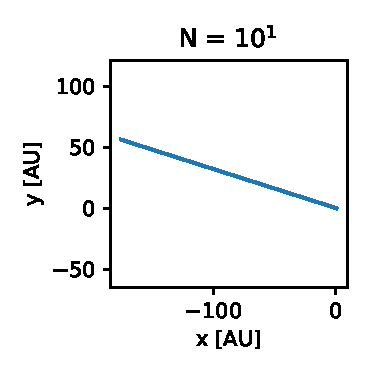
\includegraphics[width=4cm]{figs/ex_b_orbit_velocityverlet_1.pdf}}
  \subfloat[][Forward Euler]{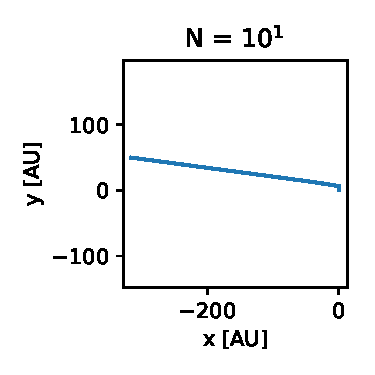
\includegraphics[width=4cm]{figs/ex_b_orbit_eulerforward_1.pdf}} 
  \subfloat[][Velocity-Verlet]{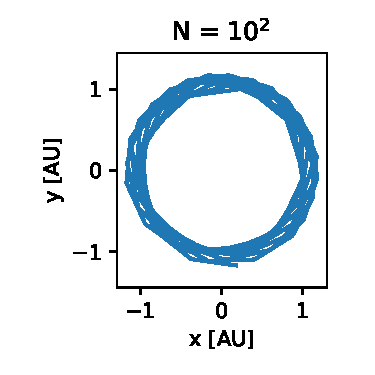
\includegraphics[width=4cm]{figs/ex_b_orbit_velocityverlet_2.pdf}}
  \subfloat[][Forward Euler]{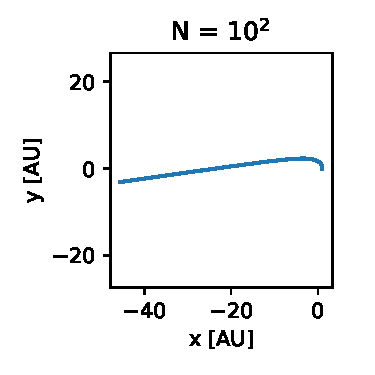
\includegraphics[width=4cm]{figs/ex_b_orbit_eulerforward_2.pdf}} 
  \\
  \subfloat[][Velocity-Verlet]{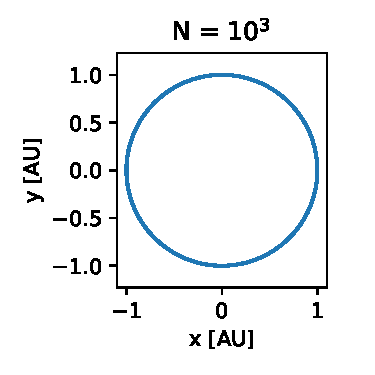
\includegraphics[width=4cm]{figs/ex_b_orbit_velocityverlet_3.pdf}}
  \subfloat[][Forward Euler]{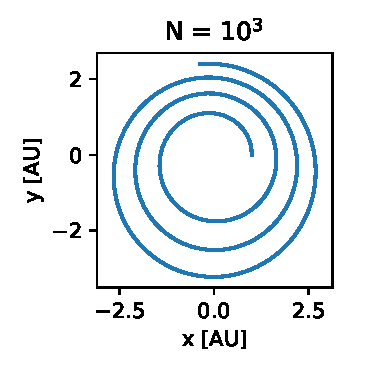
\includegraphics[width=4cm]{figs/ex_b_orbit_eulerforward_3.pdf}} 
  \subfloat[][Velocity-Verlet]{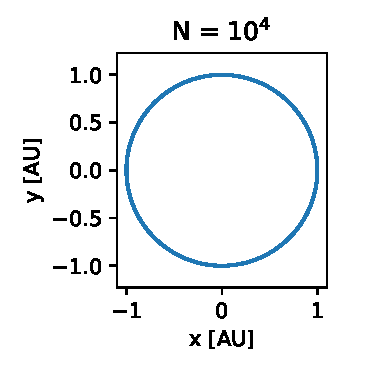
\includegraphics[width=4cm]{figs/ex_b_orbit_velocityverlet_4.pdf}}
  \subfloat[][Forward Euler]{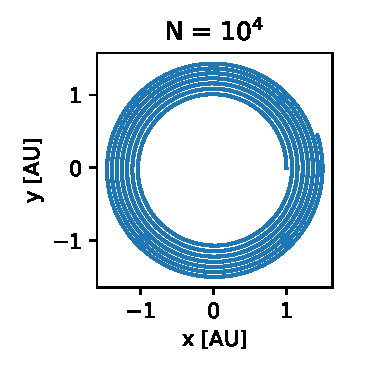
\includegraphics[width=4cm]{figs/ex_b_orbit_eulerforward_4.pdf}} 
  \\
  \subfloat[][Velocity-Verlet]{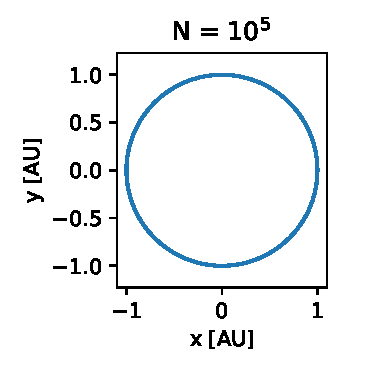
\includegraphics[width=4cm]{figs/ex_b_orbit_velocityverlet_5.pdf}}
  \subfloat[][Forward Euler]{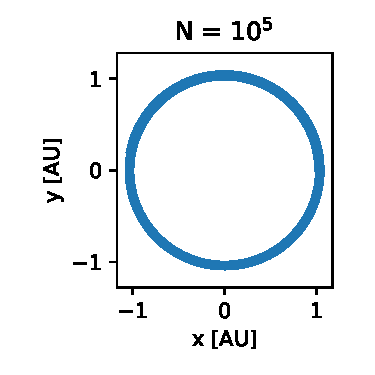
\includegraphics[width=4cm]{figs/ex_b_orbit_eulerforward_5.pdf}}
  \subfloat[][Velocity-Verlet]{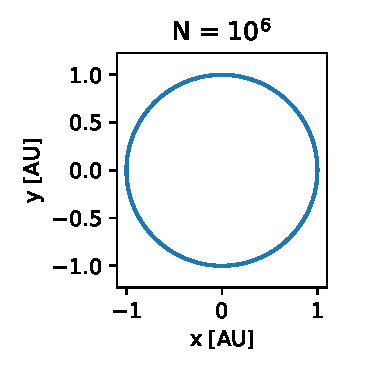
\includegraphics[width=4cm]{figs/ex_b_orbit_velocityverlet_6.pdf}}
  \subfloat[][Forward Euler]{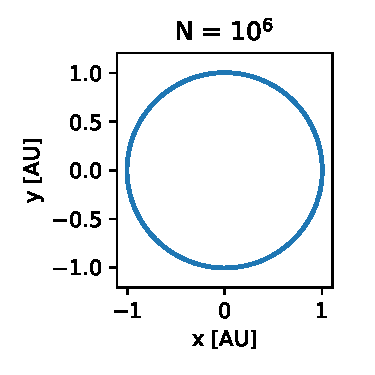
\includegraphics[width=4cm]{figs/ex_b_orbit_eulerforward_6.pdf}} 
  \caption{The orbit of earth around a stationary sun for a timeperiod of 10 Years with simulated with a varying number of integration points N (see fig titles) using the Velocity-Verlet and Forward Euler algorithms}
  \label{fig:3c_earthsun}
\end{figure*}
 
\begin{figure*}
  \center
  \subfloat[][Velocity-Verlet]{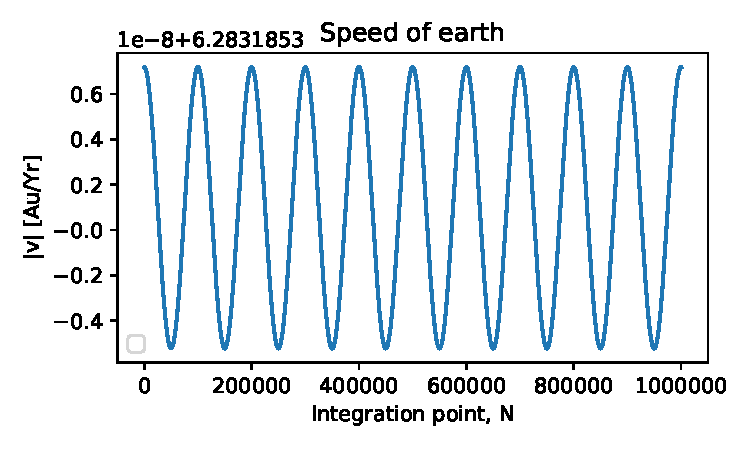
\includegraphics[width=8cm]{figs/ex_b_speed_velocityverlet_6.pdf}\label{fig:earthsun speed verlet}}
   \subfloat[][Forward Euler]{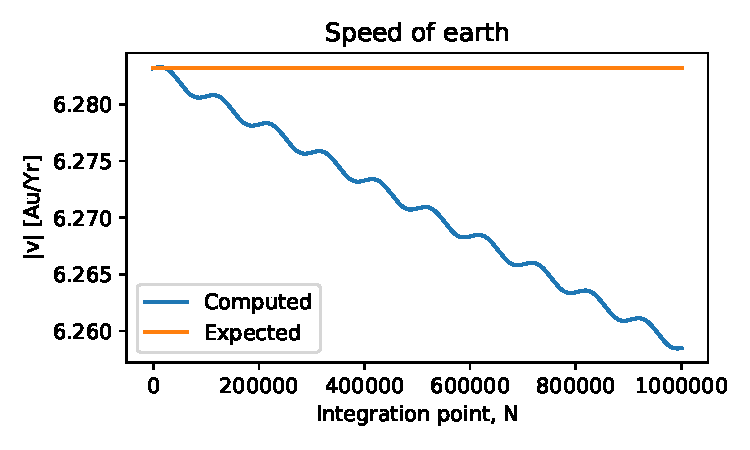
\includegraphics[width=8cm]{figs/ex_b_speed_eulerforward_6.pdf}\label{fig:earthsun speed forward euler}}
   \caption{The speed of Earth in the Earth-Sun system for solutions using the Velocity-Verlet algorithm (a) and the Forward Euler algorithm (b) in a 10 Year simulation and $N=10^6$ integration points}
   \label{fig:c_speed}
\end{figure*}
\begin{figure*}
  \center
  \subfloat[][Velocity-Verlet]{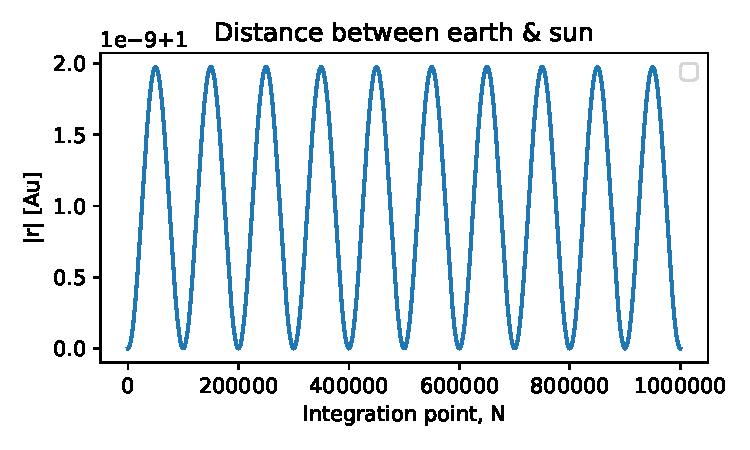
\includegraphics[width=8cm]{figs/ex_b_radius_velocityverlet_6.pdf}\label{fig:earthsun potential verlet}\label{fig:c_radius_verlet}}
   \subfloat[][Forward Euler]{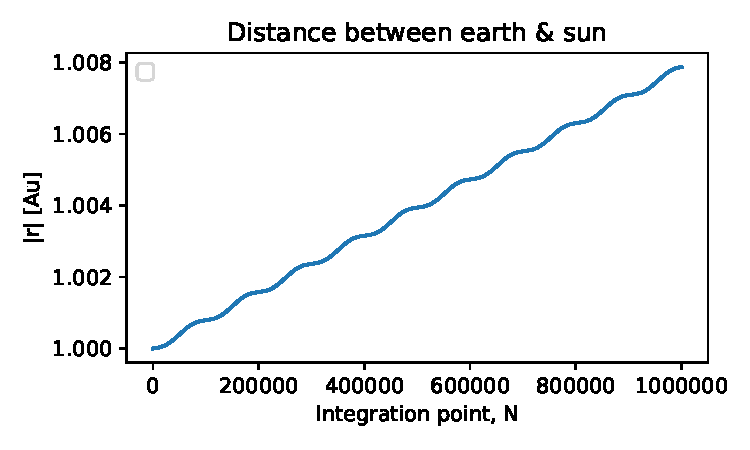
\includegraphics[width=8cm]{figs/ex_b_radius_eulerforward_6.pdf}\label{fig:earthsun potential forwardeuler}\label{fig:c_radius_euler}}
   \caption{The radius of Earth in the Earth-Sun system for solutions using the Velocity-Verlet algorithm (a) and the Forward Euler algorithm (b) in a 10 Year simulation and $N=10^6$ integration points}
   \label{fig:c_radius}
\end{figure*}
\newpage


  \subsection{Earth-Sun System}

    Working in units $M_\odot, AU, Years$ for mass, length and time respectively, i initialized a 2D system using the \lstinline{n_solver} class where the sun is fixed at the origin and the earth has initial velocity $\mathbf v_0 = (0, 2\pi)$ at position $\mathbf r_0 = (1, 0)$, corresponding to an orbit of eccentricity, $e=0$, a perfect circle.
    

    The system was then simulated for a time period of $10$ years using a different number of integration points for both the Velocity-Verlet and Forward Euler algorithms. The resulting orbits shown in Fig. \ref{fig:3c_earthsun}, shows that the Velocity-Verlet solution yields a reasonable approximate orbit for $N=10^3$ integration points, whilst the Forward Euler algorithm doesn't produce a comparable orbit until $N=10^6$ integration points. In Fig. \ref{fig:timing} we see the time it took for my program to solve this system for a selection of $N$. These numbers apply of course, only to the particular system with a fixed sun and one orbiting planet, as calculating the acceleration on more than one planets adds to the number of FLOPS.

    \begin{figure}[H]
      \center
      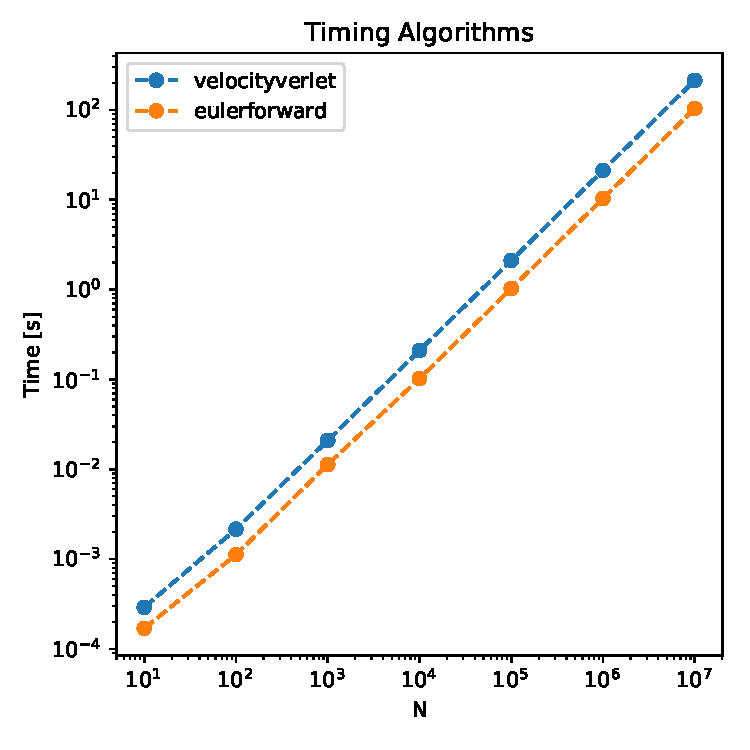
\includegraphics[width=8cm]{figs/timing_earthsun.pdf}
      \caption{Time taken to solve the Earth-Sun system for different number of integration points for $t_n=10\, Yr$}
      \label{fig:timing}
    \end{figure}

    In Figures \ref{fig:c_speed}, \ref{fig:c_radius} we see how the speed and radius evolves throughout the integration points for $N=10^6$, and most notably, how they change. As mentioned prior, for the set of initial conditions used, we expect a perfectly circular orbit, but also constant speed. Looking at Figures \ref{fig:earthsun speed forward euler}, \ref{fig:c_radius_euler}, corresponding to the Forward Euler solution, that the earth is slightly drifting away from the sun, whilst losing speed, which further implies that both the potential and kinetic energy in the system has not been conserved\footnote{Because $E_k \propto v^2$ and $E_p\propto -\frac{1}{r}$}. Now we turn to Figures \ref{fig:earthsun speed verlet}, \ref{fig:c_radius_verlet}, corresponding to the Velocity-Verlet solution, where we see a periodic, but seemingly constant behavior of both the radius and speed, meaning that on average the energy of the system is conserved. Since the angular momentum is proportional to the product of the speed and radius, it follows that it is conserved and not conserved for the Verlet and Euler algorithms respectively.

    \begin{figure}[H]
      \center
      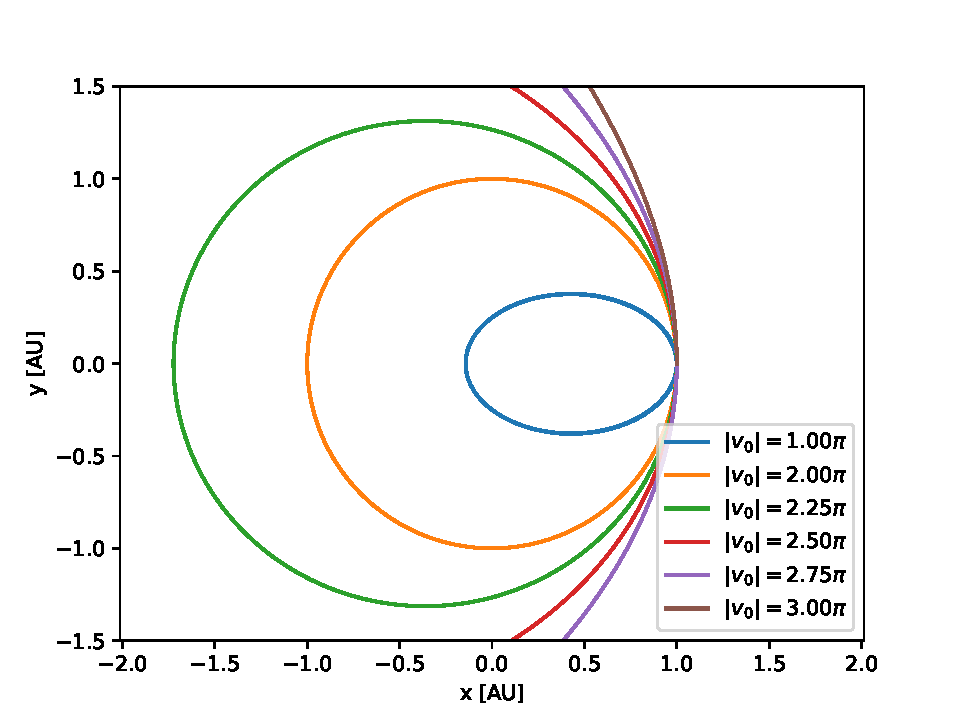
\includegraphics[width=8cm]{figs/ex_d_escape.pdf}
      \caption{The trajectories of Earth in the Earth-Sun system for different initial velocities and $N=5\cdot 10^5$ integration points over a $50$ year simulation.}
      \label{fig: escapevel}
    \end{figure}

    \subsubsection{Escape Velocity}


    In Fig. \ref{fig: escapevel} we see the trajectories resultant of different initial speeds, $|v_0|$. See that the only orbit which isn't closed is that for $|v_0|=3\pi$, meaning the escape velocity is in the interval $[2.75\pi, 3\pi]$. From Eqn. \ref{eqn:escapevel} we find that the theoretical escape velocity is $\sqrt{8}\pi$, matching our result. Of course this is rather trivial, so i now point you to \footnote{Which is found after the main text, because figure placement isn't always the easiest when producing a document in revtex}Fig. \ref{fig: escapevel varbeta}, in which we see what happens to the same problem in a universe where the force of gravity is proportional to $r^{-\beta}, \, \beta \in [2, 3]$, instead of $|\mathbf F| \propto r^{-2}$. What is very interesting to note, is that $|v_0|=2\pi$ seemingly remains a stable orbit in the selected values for which i simulated, whilst all other 'surrounding' change drastically, taking particular note of the interesting pattern that emerges from $\beta=2.5, \, |v_0| = 1\pi$. 

    \begin{figure*}[h!p]
      \subfloat[][$\beta = 2.5$]{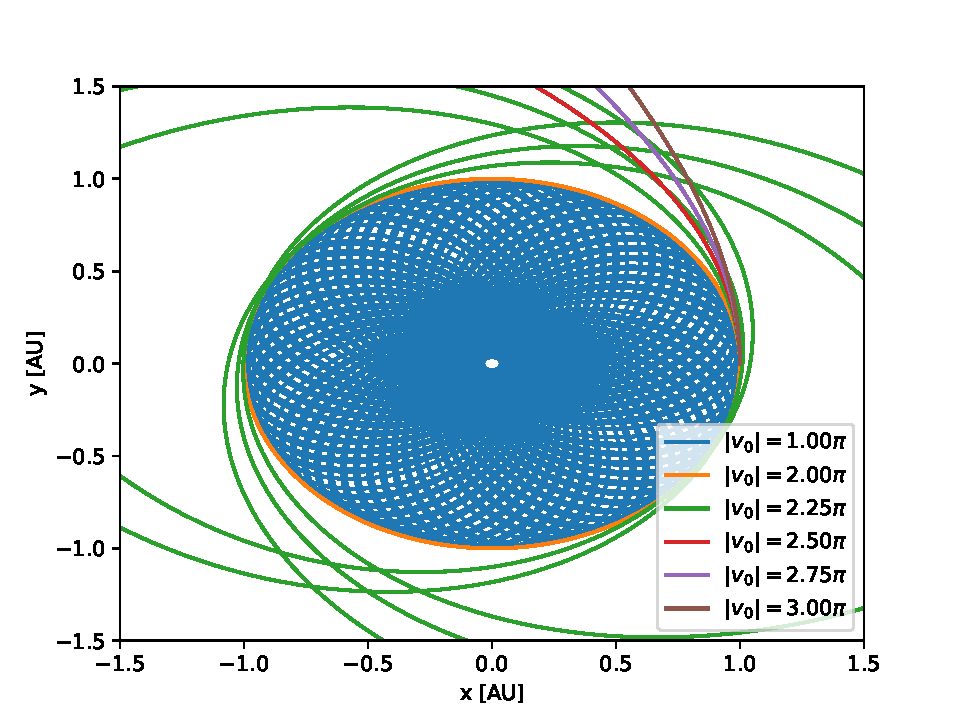
\includegraphics[width=8cm]{figs/ex_d_escape_25.pdf}}
      \subfloat[][$\beta = 2.75$]{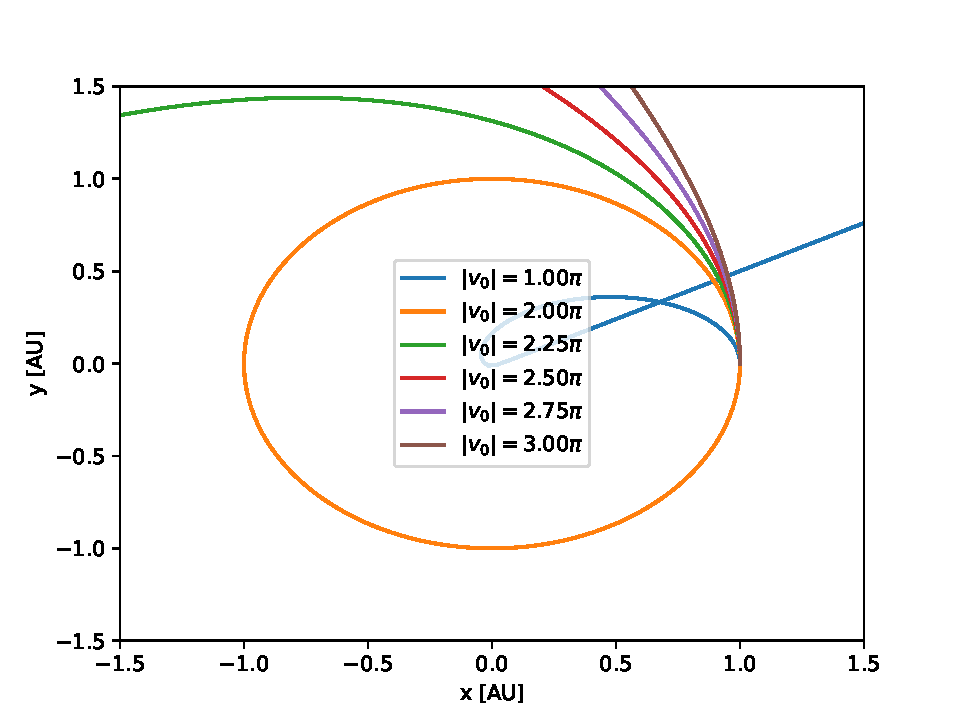
\includegraphics[width=8cm]{figs/ex_d_escape_275.pdf}}\\
      \subfloat[][$\beta = 2.9$]{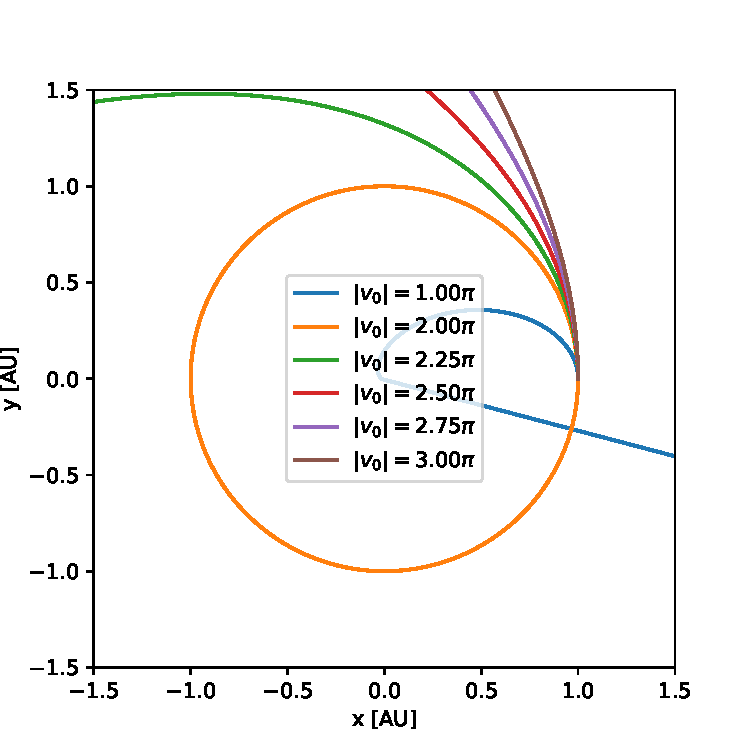
\includegraphics[width=8cm]{figs/ex_d_escape_29.pdf}}
      \subfloat[][$\beta = 3$]{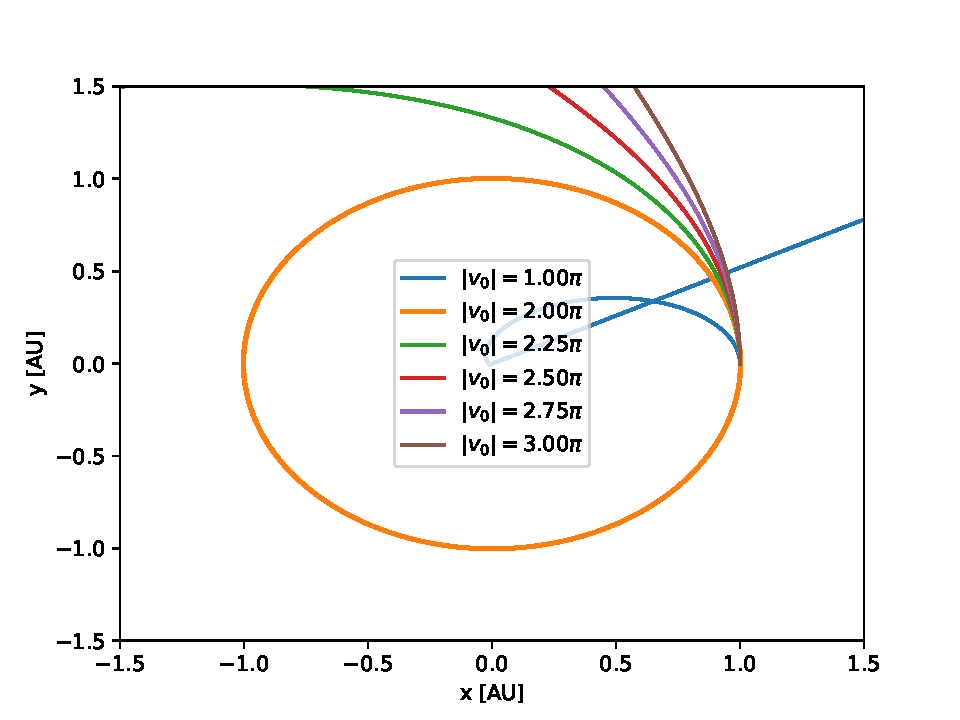
\includegraphics[width=8cm]{figs/ex_d_escape_3.pdf}}
      \caption{Trajectories in the earth-sun system initialized $1\,$AU away from the sun with modified laws of gravity such that $|\mathbf F|\propto r^{-\beta}$}
      \label{fig: escapevel varbeta}
    \end{figure*}

\subsection{3-Body problem}
  Fetching initial conditions from the Horizons\footnote{\url{https://ssd.jpl.nasa.gov/horizons.cgi}, for which astroquery provides an easy way to import data into python, further simplified by my script \lstinline{get_initconds.py}} system hosted by JPL at NASA, i simulated the trajectory of Earth and Jupiter orbiting around a fixed sun. As the data is in 3 dimensions, this also proved a great time to test flexibility of \lstinline{n_solver}, which as expected worked just as well when fed 3D data, without having to make any adjustments to the way in which the code is called. The trajectory for a 30 Year simulation with $N=10^6$ integration points is presented in Fig \ref{fig:jupiter_1_30}.
  The resultant orbits are seemingly uniform, and stable within the time frame of the solution.

  \begin{figure}[H]
    \center
    \subfloat[][$M_{jupiter}$, $t=30$ Yr]{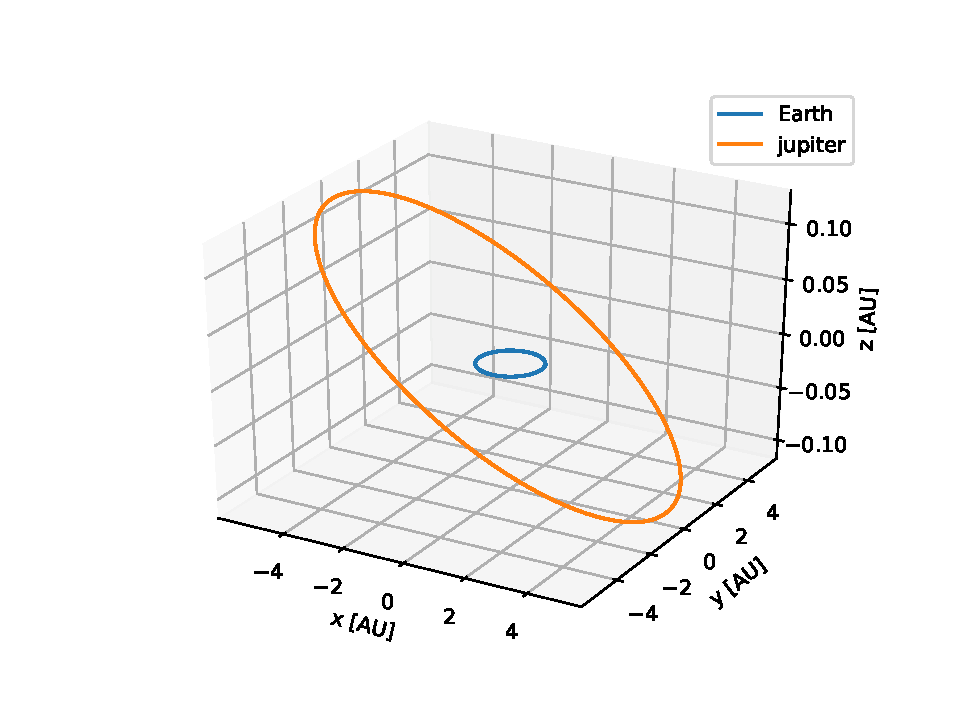
\includegraphics[width=8cm]{figs/exe_earth_jupiter_1_30yrs.pdf}\label{fig:jupiter_1_30}}\\
    \subfloat[][$10M_{jupiter}$, $t=30$ Yr]{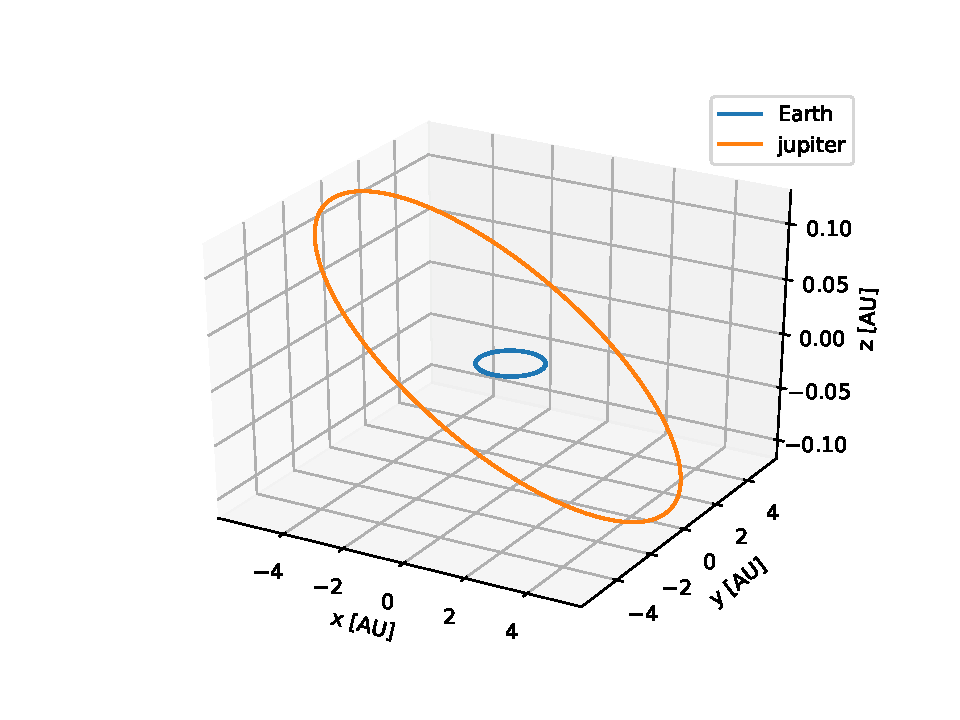
\includegraphics[width=8cm]{figs/exe_earth_jupiter_10_30yrs.pdf}}\\
    \subfloat[][$10^3M_{jupiter}$, $t=15$ Yr]{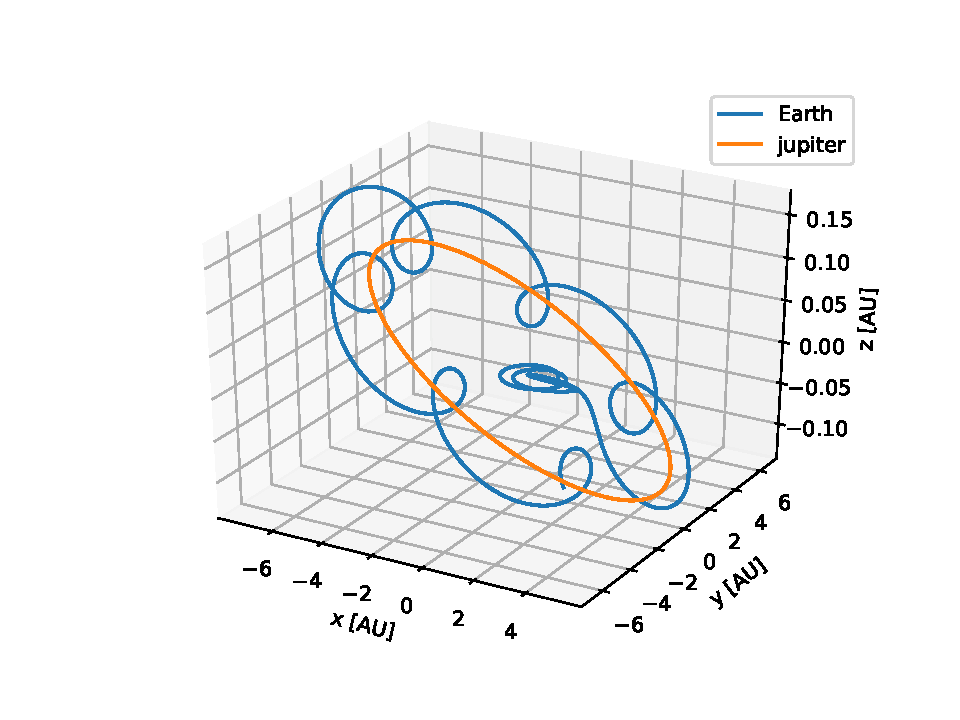
\includegraphics[width=8cm]{figs/exe_earth_jupiter_1000_15yrs.pdf}}
    \caption{Trajectories for earth and jupiter in the 3-body system with fixed sun at the origin, with the mass of jupiter multiplied by a factor 10 (b) and $10^3$ (c) solved with $N=10^6$ integration points}
    \label{fig:exe jupiter mass increase}
  \end{figure}
  
  \newpage

  Now, we will look at what the system would look like if the mass of Jupiter was increased by a factor 10, and 1000, also presented in Fig. \ref{fig:exe jupiter mass increase}. We see that the resultant trajectory with the mass of Jupiter increased by a factor 10 looks much the same as what we saw in Fig. \ref{fig:jupiter_1_30}, but increasing the mass by a factor 1000 throws the system out of control and eventually slingshots the earth far away from the system, which can be seen in \footnote{Again, after the main text has ended}Fig. \ref{fig:ex_e earth slingshot}. Whilst a fun exercise, it is important to note that this simulation is not necessarily physically realistic, not because of the instantaneous mass increase of Jupiter, but because the planets are treated as point particles, which only interact via gravity. A more realistic outcome of this scenario would be that earth crashes into either the sun and Jupiter in a horrid, and violent fashion.

\subsection{Simulating the Solar system}
  As a final example of simulations using Newtonian gravity, i present a simulation of all the major bodies in the solar system in motion about the barycenter\footnote{Center of mass in an n-body system} in Fig \ref{fig:solarsystem}, once again having fetched the initial conditions from the Horizons system.
  Pluto, and other smaller celestial objects could very easily be added thanks to the script i wrote, \lstinline{get_initconds.py}, which fetches initial conditions using the Astroquery python package. However, i opted not to, simply because it would add further "clutter" to a figure already lacking in any significant detail.


\begin{figure}[H]
  \center
  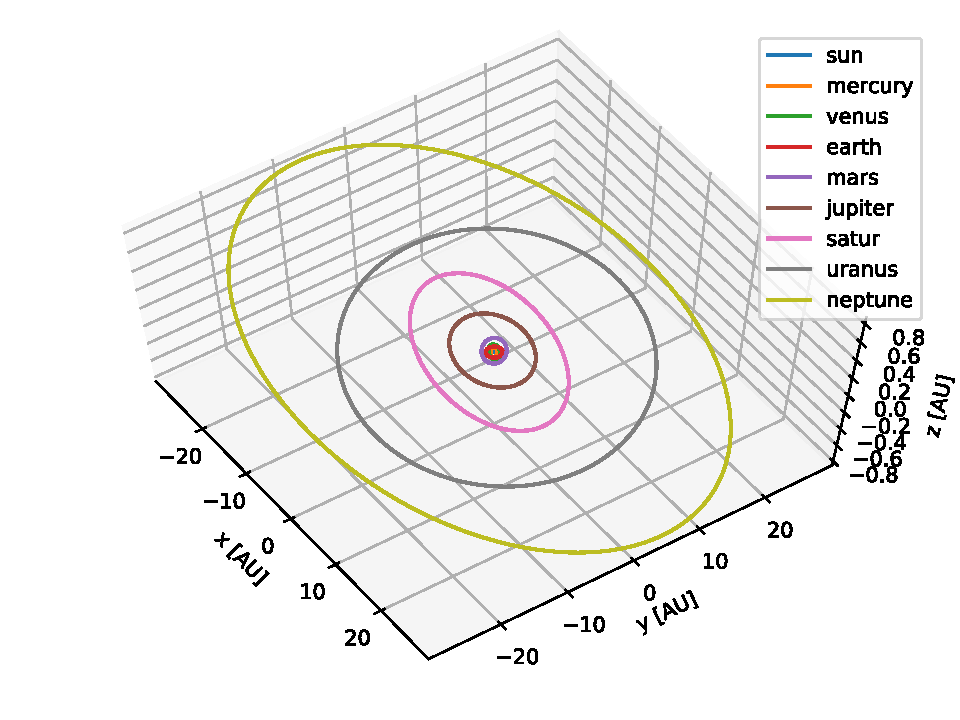
\includegraphics[width=8cm]{figs/all_bodies.pdf}
  \caption{Simulation of the major bodies within the solar system for 165 Years and $N=10^6$ integration points using initial conditions from Horizons}
  \label{fig:solarsystem}
\end{figure}


\subsection{The perihelion precession of Mercury}
  In order to test the relativistic correction proposed in Eqn. \ref{eqn:relativistic correction} i extended \lstinline{n_solver} by adding a method which solves the 2-body problem with a stationary sun. I then initialized the system with mercury at its perihelion, $0.3075\,\textup{AU}$ away from the sun with speed $12.44\, \textup{AU Yr}^{-1}$ \cite{problem_set}. I simulated the system for $100$ years with $N=10^8$ integration points, which took my computer $7131.14\,\textup s$, just under 2 hours to solve. I then found the radius between the sun and mercury for all $t$ and looped backwards, finding the first minima. Having found the index in which the mercury was previously at its perihelion I then found that the angle of precession to be $5.09\,\textup{rad}$, or $10.51"$, significantly lower than what is observed experimentally.

  This could be due to either the simplification in the model, not including the other planets in the system, or it could simply be an error in my implementation of the system. As this simulation takes such a significant amount of time to run on my computer, it simply isn't feasible for me to explore this problem much further.


\section{Conclusions}
  We have seen how the choice of numerical method when solving ODE's is of great importance when analyzing numerical results, as one might draw incorrect conclusions when inferring about the time evolution of the energy of a system when using non-conservative methods, which the Forward Euler algorithm turned out to be in this problem. Further, whilst more computationally expensive per iteration, the Velocity-Verlet proves to be the cheaper method when accounting for its quick convergence when compared to the Forward Euler method.

  Lastly, in regards to object orientation, i find that many of the supposed 'benefits' of this type of development simply does not apply to numerical computation, regardless of its usefulness in other scenarios. Abstracting what is otherwise simple, numerical computations which we as physicists are very much familiar is nonsensical in my opinion. If i were to define my own, special data-types to be operated on by numerical algorithms, that would only serve to decrease the flexibility of my algorithms by requiring to define new, similar data types which could be operated on in a similar fashion if i were to utilize the program to another problem.

  Of course, the aforementioned problems does not strictly apply to my class\footnote{which just as easily could have been implemented in a strictly functional approach}, \lstinline{n_solver}, which should work effortlessly for different systems, given new methods for the governing forces.


\begin{thebibliography}{99}
%\bibitem{lecture_notes} M.~Hjorth-Jensen, Computational Physics - Lecture Notes 2015, (2015).
\bibitem{ode_lecture} M.~Hjorth-Jensen, Ordinary differential equations - Computational Physics Lectures (2017)
\bibitem{problem_set} M.~Hjorth-Jensen, Building a model for the solar system using ordinary differ-
ential equations - Project 3 (2018)
\bibitem{elem} A.~Malthe-Sørenssen, Elementary Mechanics Using Python (2015)
\end{thebibliography}


  \begin{figure*}[h!]
    \center
    \subfloat[][t=5 years]{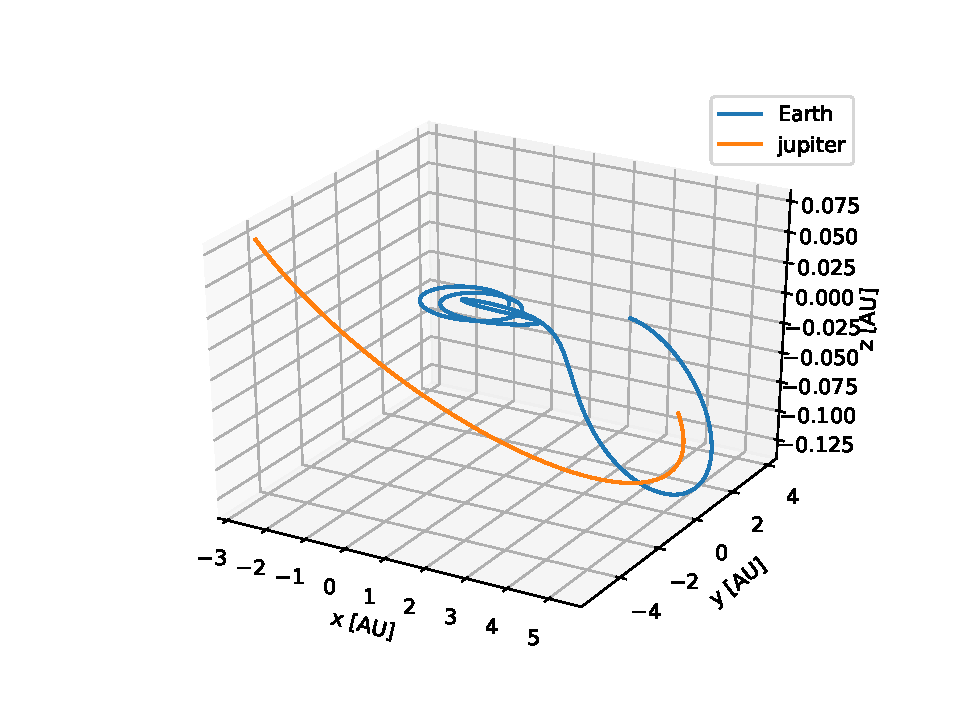
\includegraphics[width=8cm]{figs/exe_earth_jupiter_1000_5yrs.pdf}}
    \subfloat[][t=10 years]{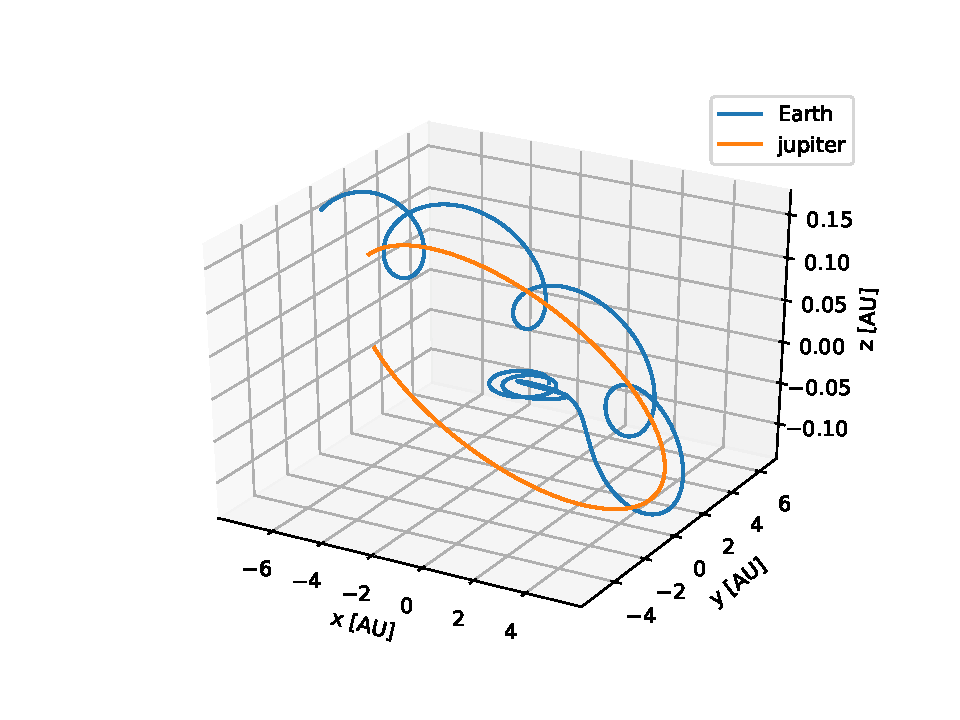
\includegraphics[width=8cm]{figs/exe_earth_jupiter_1000_10yrs.pdf}}\\
    \subfloat[][t=15 years]{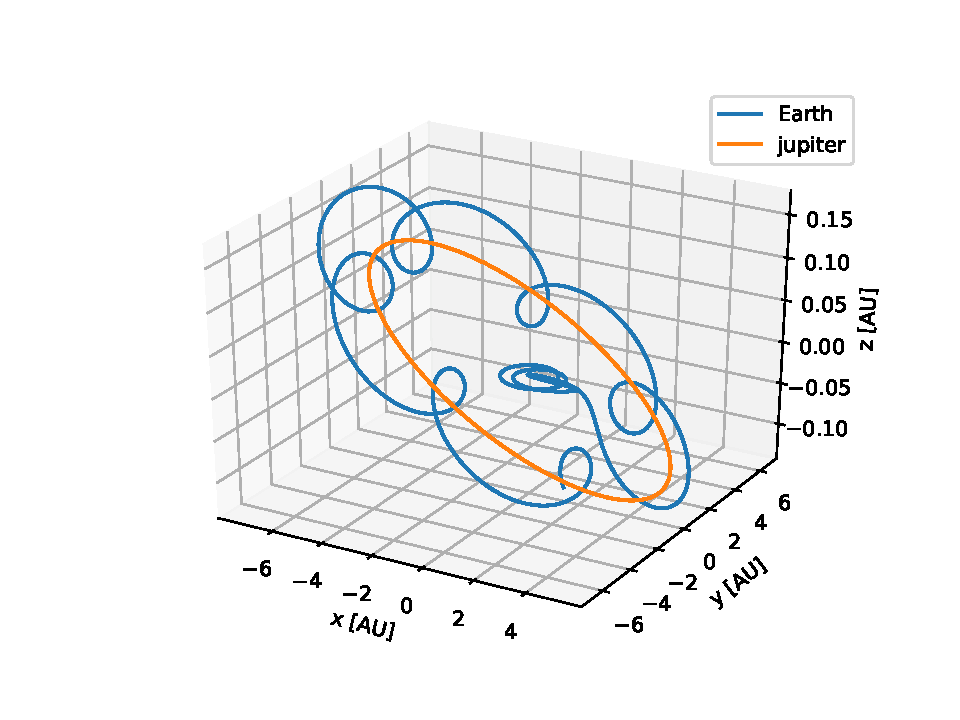
\includegraphics[width=8cm]{figs/exe_earth_jupiter_1000_15yrs.pdf}}
    \subfloat[][t=20 years]{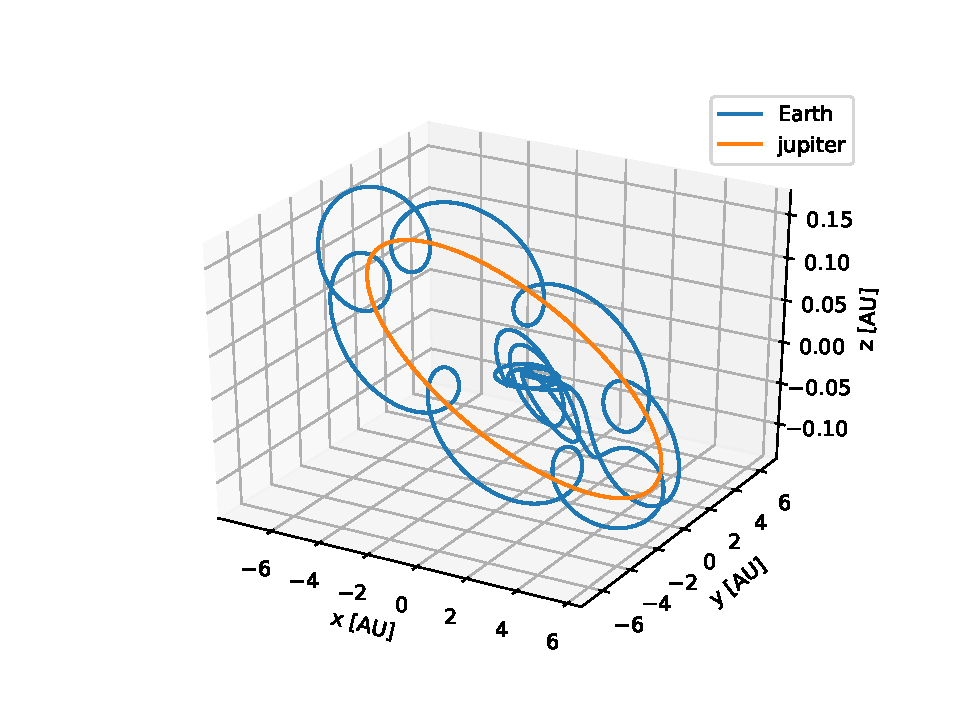
\includegraphics[width=8cm]{figs/exe_earth_jupiter_1000_20yrs.pdf}}\\
    \subfloat[][t=20 years]{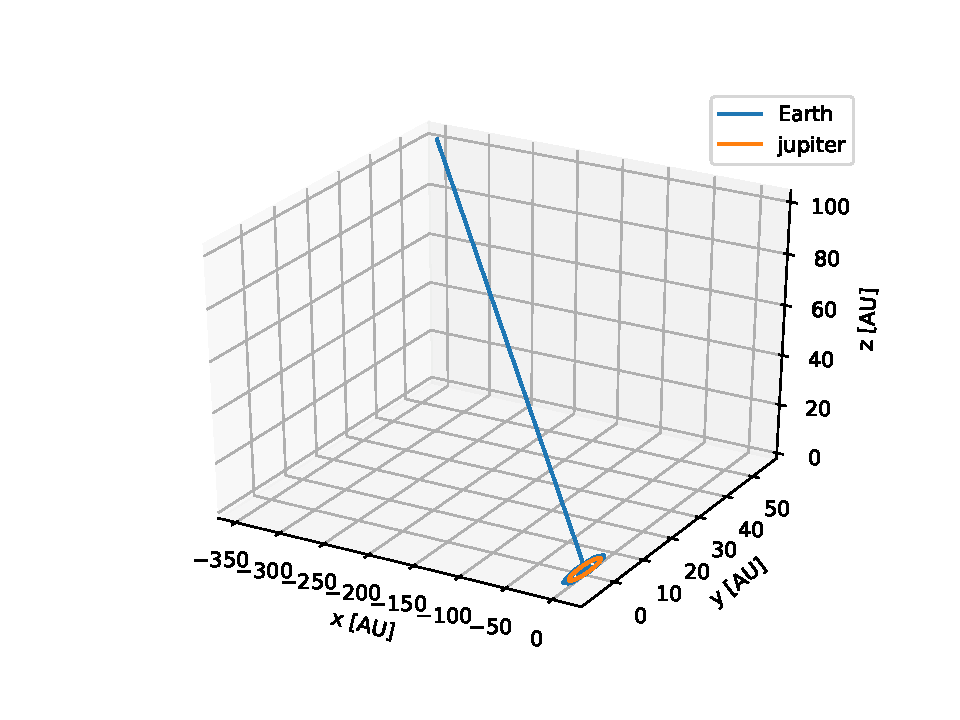
\includegraphics[width=8cm]{figs/exe_earth_jupiter_1000_25yrs.pdf}}
    \subfloat[][t=20 years]{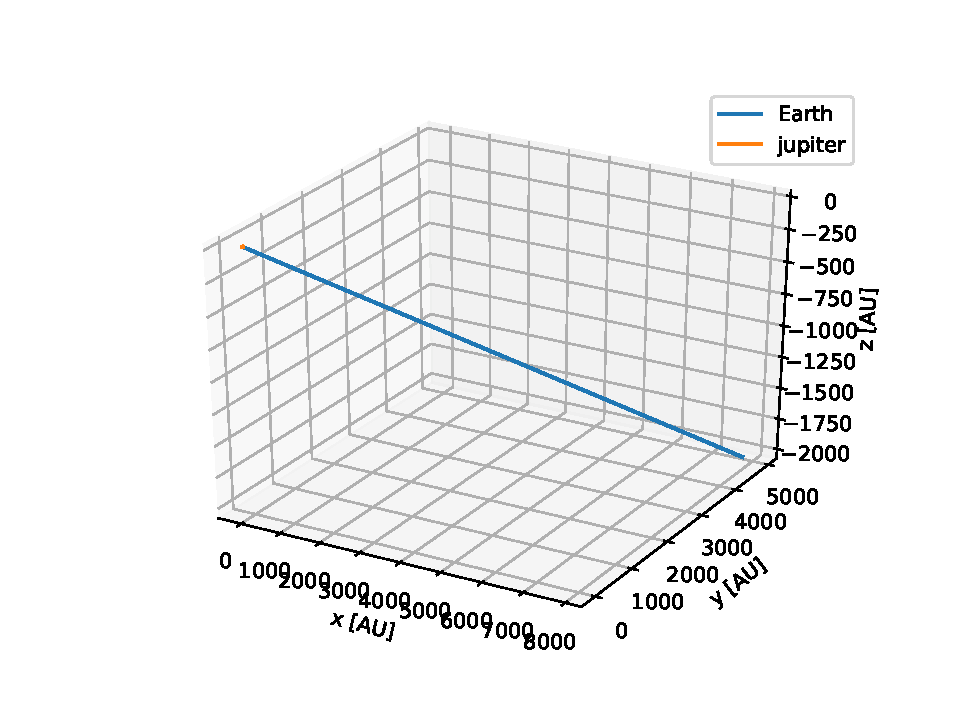
\includegraphics[width=8cm]{figs/exe_earth_jupiter_1000_30yrs.pdf}}
    \caption{Trajectories of Earth and Jupiter with the sun fixed at the center and jupiters mass multiplied by $\times 1000$ at different times, simulated with $N=10^6$ integration points}
    \label{fig:ex_e earth slingshot}
  \end{figure*}


\begin{figure*}[h!]
  \center
  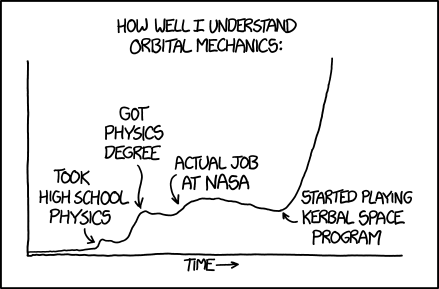
\includegraphics[scale=0.5]{figs/orbital_mechanics.png}
  \caption{To wrap things up i present to you a highly relevant xkcd comic}
\end{figure*}

\end{document}  